\section{Datasets description}
The original bike sharing dataset\footnote{it is possible to download it from this web page: \url{https://www.kaggle.com/datasets/vineethakkinapalli/citibike-bike-sharingnewyork-cityjan-to-apr-2021}.} comes from the website Kaggle and contains the bicycle rental information in \num{2020} of the company Citi Bike in Jersey City (figure \ref{Train_map}). Citi Bike is a privately owned public bicycle sharing system serving the New York City boroughs of the Bronx, Brooklyn, Manhattan, and Queens, as well as Jersey City. The weather dataset, instead, contains the most significant meteorological variables' time series about NYC in \num{2020} and comes from the historical weather data database that the website Visual Crossing\footnote{more information at this web site: \url{https://www.visualcrossing.com/weather-data}.} makes available for the users. Moreover, we have constructed two logical dummy variables to describe the weekends and events that have occurred in New York City in \num{2020}, i.e. the US federal holidays and the lockdown due to the COVID-\num{19} pandemic.
Through a preliminary data processing work, we have extracted from the original datasets the variables of our interest by grouping data to obtain daily and hourly information. In the following paragraphs we have summarized some information about them.

\subsection{Bike sharing variables}
This partition contains all the information relating to the bike rental: 
\begin{itemize}
	\item \textbf{pickups counter}: number of pickups at a rental station;
	\item \textbf{mean trip duration}: mean rental time of a user who picks-up a bike at a rental station;
	\item \textbf{mean users age}: mean age of a user who picks-up a bike at a rental station;
	\item \textbf{male counter}: number of males who pick-up a bike at a rental station;
	\item \textbf{female counter}: number of women who pick-up a bike at a rental station;
	\item \textbf{unknown gender counter}: number  of people who have not specify their gender who pick-up a bike at a rental station;
	\item \textbf{subscribers counter}: number of customers who pick-up a bike at a rental station having an annual subscription;
	\item \textbf{customers counter}: number of customers who pick-up a bike at a rental station having a \num{4}-hour pass or a \num{3}-day pass;
	\item \textbf{distance}: indicates the distance between a rental station and the nearest train or subway station in \unit{\kilo\meter} (figure \ref{Distances_map}).
	
\end{itemize}
All these variables are both space-variant and time-variant, except for the distance that is a time-invariant covariate which we have obtained by carrying out an in-depth analysis of public transport network in Jersey City.

\begin{figure}[h!]
	\centering
	\subfigure[]{\label{Distances_map}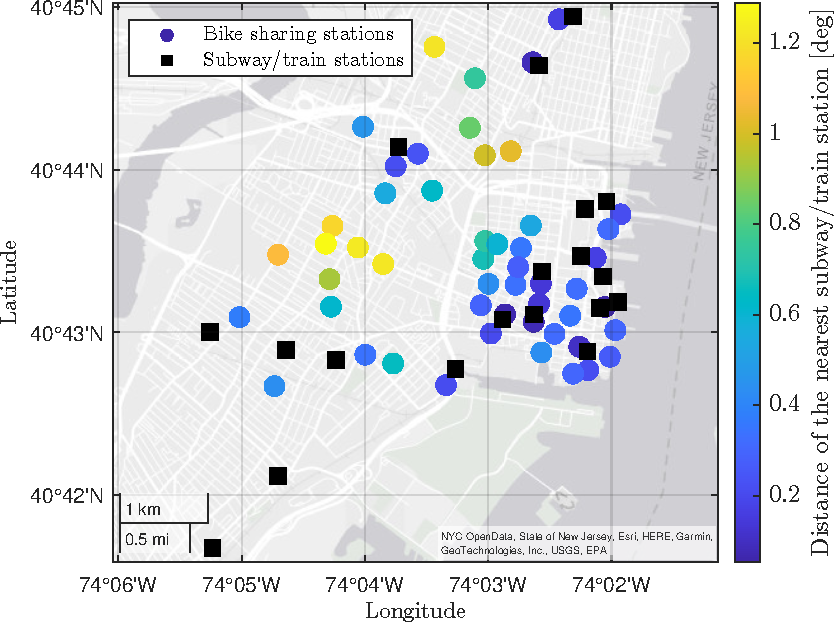
\includegraphics[height=172px]{Images/Dataset description/Chosen/Distances_map}}\quad
	\subfigure[]{\label{Train_map}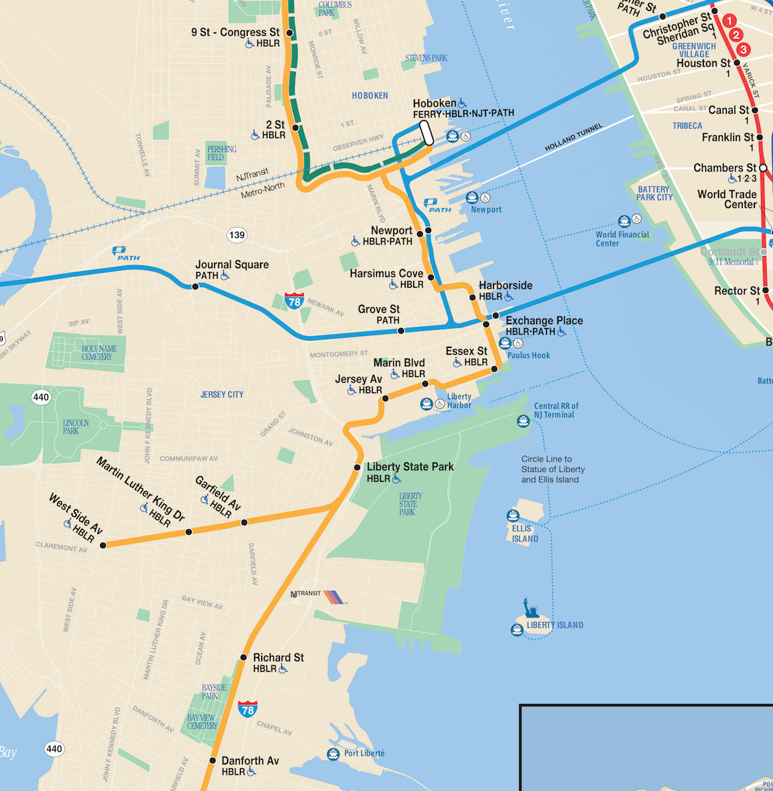
\includegraphics[height=172px]{Images/Dataset description/Chosen/Train_map}}\quad
	\caption[]{map of the bike rental stations and of the nearest subway/train stations (a) and map of the public transport network in Jersey City (b); in particular the blue line indicates the path of the public transport service which reaches Manhattan, instead the yellow line those which extends over the entire Jersey area.}
	\label{Maps}
\end{figure} 

\subsection{Weather variables}
The weather frequency variables that Visual Crossing provides to users with daily or hourly frequency are:
\begin{itemize}
	\item \textbf{mean temperature}: in \unit{\degreeCelsius};
	\item \textbf{mean feels-like temperature}: in \unit{\degreeCelsius} (figure \ref{T_plot});
	\item \textbf{relative humidity}: in percentage (figure \ref{Humidity_box});
	\item \textbf{rainfall}: in \unit{\milli\meter} (figure \ref{Rain_plot});
	\item \textbf{snowfall}: in \unit{\centi\meter};
	\item \textbf{mean wind speed}: in \unit{\kilo\meter/\hour} (figure \ref{Wind_box});
	\item \textbf{cloud cover}: percentage of covered sky (figure \ref{Cloud_box});
	\item \textbf{visibility}: maximum distance of visibility in \unit{\kilo\meter}. If the field of vision is greater than \SI{16}{\kilo\meter}, then the visibility value remains this one;
	\item \textbf{UV index}: indicates the energy of UV rays from \num{1} to \num{10} (figure \ref{UV_box}).
\end{itemize}
Weather variables are time-variant, but space-invariant because the \num{51} rental stations belong to the same geographical are. In table \ref{Weather_stats} we have summarized some of the most important statistics indicators to describe the distribution of each weather variable.

\begin{table}[h!]
	\centering
	\renewcommand\arraystretch{1.3}
	\begin{tabular}{c|c|c|c|c|c|c|c|c}
		\hline
		\textit{} & \textit{Min.} & \textit{Max.} & \textit{Mean} & \textit{Median} & \textit{Std} & \textit{Skew.}  & \textit{Kurt.} & \textit{R2} \\
		\hline
		\textbf{Temperature} & \num{-3.50} & \num{30.40} & \num{14.55} & \num{14} & \num{8.50} & \num{0.04} & \num{1.86} & \num{0.67} \\
		\hline
		\textbf{Feels-like temp.} & \num{-7.70} & \num{33.30} & \num{13.81} & \num{13.90} & \num{9.80} & \num{0.04} & \num{1.96} & \num{0.66} \\
		\hline
		\textbf{Humidity} & \num{35.10} & \num{93.50} & \num{65.28} & \num{66.10} & \num{13.78} & \num{0.08} & \num{2.18} & $\sim 0$ \\
		\hline
		\textbf{Rainfall} & \num{0} & \num{31.03} & \num{1.11} & \num{0} & \num{3.44} & \num{5.44} & \num{39.01} & \num{-0.06} \\
		\hline
		\textbf{Snowfall} & \num{0} & \num{157.50} & \num{0.78} & \num{0} & \num{9.61} & \num{14.45} & \num{219.19} & \num{-0.05} \\
		\hline
		\textbf{Wind speed} & \num{9.90} & \num{47.80} & \num{20.64} & \num{19.90} & \num{6.89} & \num{0.98} & \num{3.90} & \num{-0.26} \\
		\hline
		\textbf{Cloud cover} & \num{0.10} & \num{100} & \num{39.45} & \num{37.15} & \num{29.79} & \num{0.35} &\num{ 1.95} & \num{-0.33} \\
		\hline
		\textbf{Visibility} & \num{6.50} & \num{16} & \num{15.29} & \num{16} & \num{1.54} & \num{-2.99} & \num{12.83} & \num{0.24} \\
		\hline
		\textbf{UV index} & \num{ 0} & \num{10} & \num{5.92} & \num{6} & \num{2.88} & \num{-0.21} & \num{1.84} & \num{0.46} \\
		\hline
	\end{tabular}
	\caption{main statistics concerning weather variables. The R2 index describes the linear correlation between a meteorological covariate and the mean number of daily pickups.}
	\label{Weather_stats}
\end{table}

\begin{figure}[h!]
	\centering
	\subfigure[]{\label{T_plot}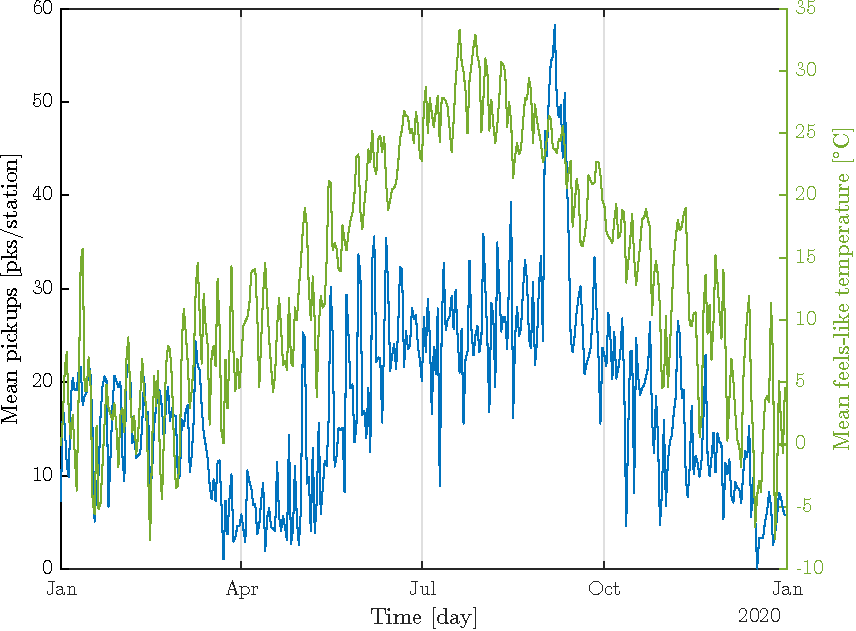
\includegraphics[height=172px]{Images/Dataset description/Chosen/Mean_feels_like_temperature_plot}}\quad
	\subfigure[]{\label{Rain_plot}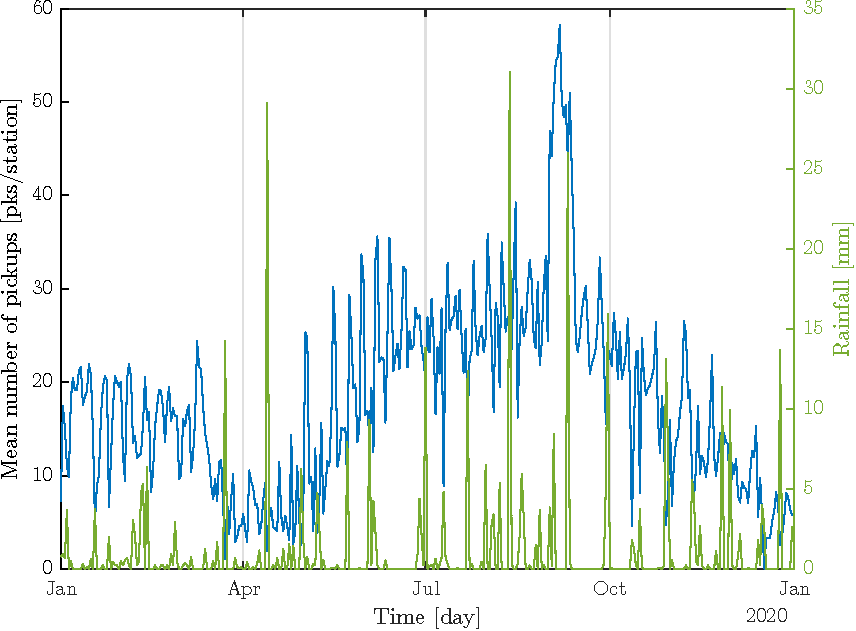
\includegraphics[height=172px]{Images/Dataset description/Chosen/Rainfall_plot}}\quad
	\caption{comparison between the trend of the mean number of daily pickups calculated on the entire bike sharing network and two weather variables, i.e. the mean daily feels-like temperature (a) and the daily rainfall (b). Through these plots we can see that temperature has a positive effects on rentals, instead rainfall a negative impact.}
\end{figure}

\begin{figure}[h!]
	\centering
	\subfigure[]{\label{Humidity_box}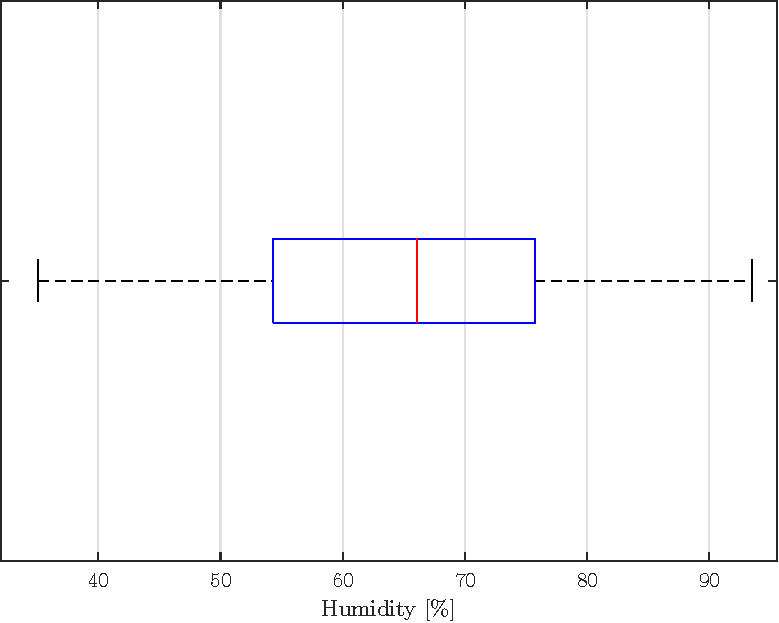
\includegraphics[height=172px]{Images/Dataset description/Chosen/Humidity_box}}\quad
	\subfigure[]{\label{Wind_box}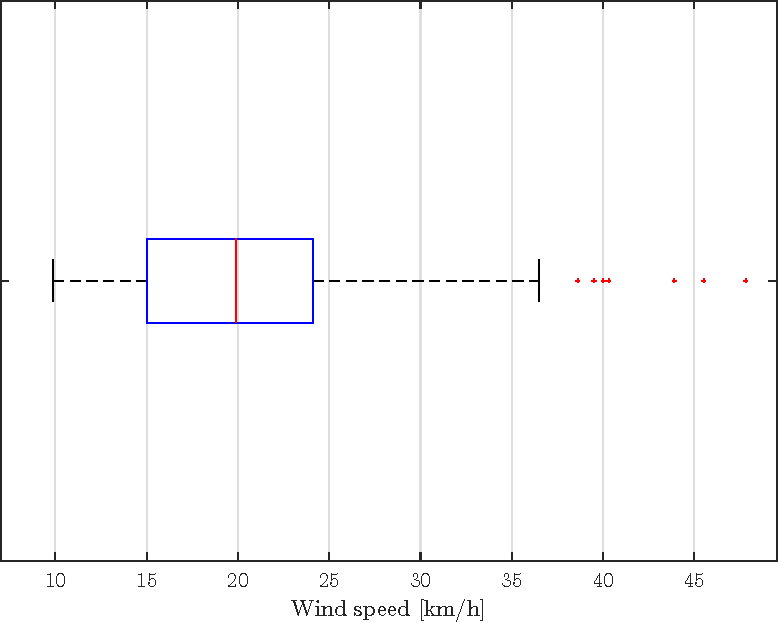
\includegraphics[height=172px]{Images/Dataset description/Chosen/Wind_speed_box}}\quad
	\subfigure[]{\label{Cloud_box}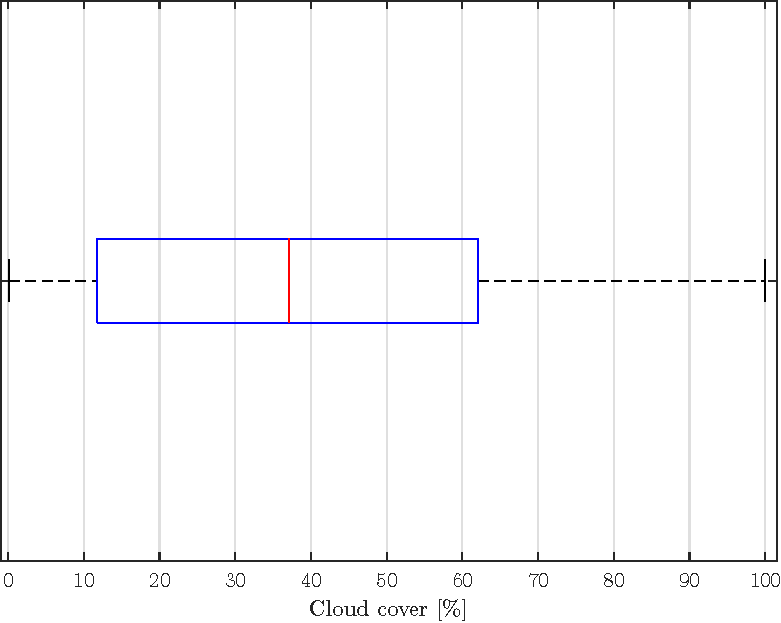
\includegraphics[height=172px]{Images/Dataset description/Chosen/Cloud_cover_box}}\quad
	\subfigure[]{\label{UV_box}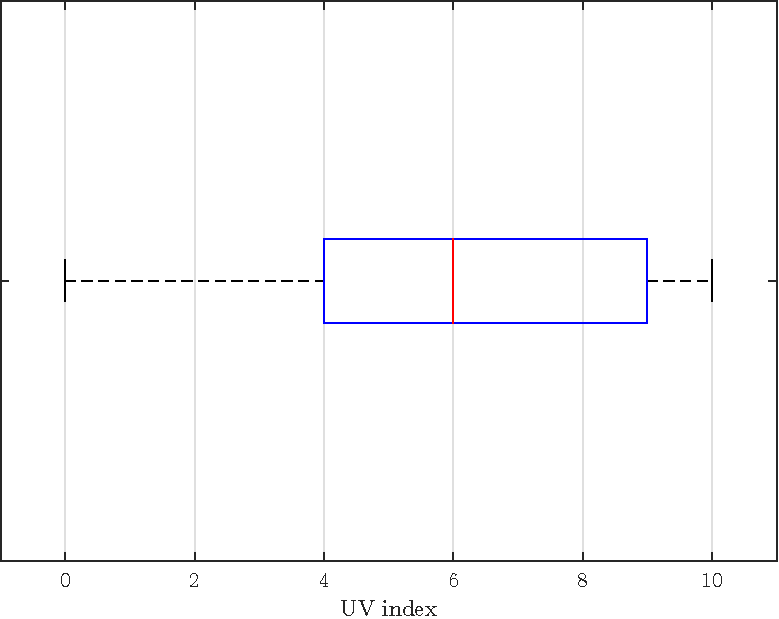
\includegraphics[height=172px]{Images/Dataset description/Chosen/UV_index_box}}\quad
	\caption{box-plots of some weather variables.}
\end{figure}

\subsection{Dummy variables}
We have hypothesized that not only weather may influence the demand of bicycle rentals, but also some events could provide their contribute, in particular the lockdown due to the COVID-\num{19} pandemicand the US federal holidays. For this reason we have defined the following binary dummy variables:
\begin{itemize}
	\item \textbf{lockdown}: this is equal to \num{1} if that day of \num{2020} there was the lockdown, \num{0} otherwise (figure \ref{Trend_ld});
	\item \textbf{weekends and holidays}: is equal to \num{1} if that day was Saturday, Sunday or a festive day, \num{0} otherwise (figure \ref{Trend_sundays}).
\end{itemize}
Dummy variables are time-variant, but space-invariant.

\begin{figure}[h!]
	\centering
	\centering
	\subfigure[]{\label{Trend_ld}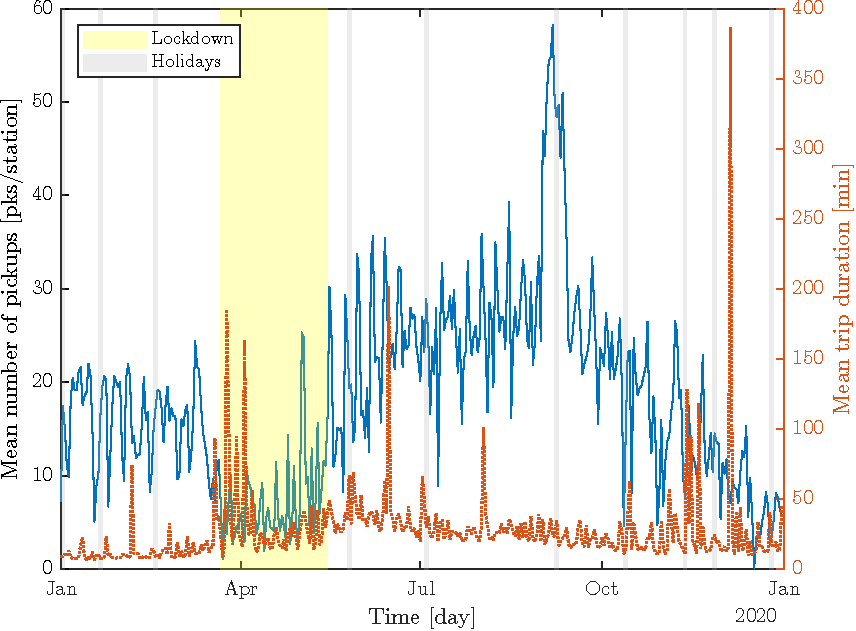
\includegraphics[height=172px]{Images/Dataset description/Chosen/Trend_ld}}\quad
	\subfigure[]{\label{Trend_sundays}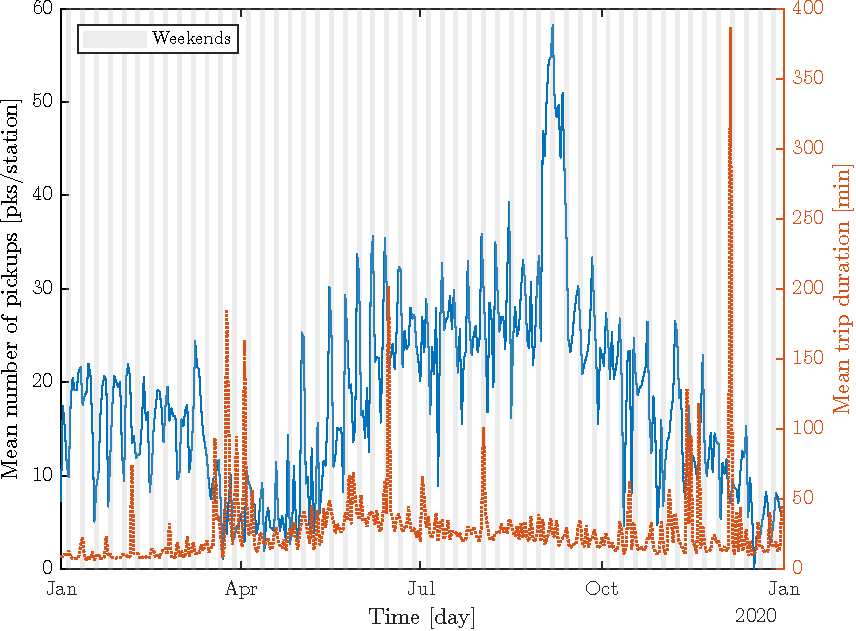
\includegraphics[height=172px]{Images/Dataset description/Chosen/Trend_sundays}}\quad
	\caption{in both graphs we can note as events influence the mean number of daily rentals. During the lockdown, in fact, there was not the possible to leave own home, instead in the weekends or during holidays a pickups' peak, either positive or negative, occurs.}
\end{figure}